% Created 2021-01-21
% Intended LaTeX compiler: pdflatex
\documentclass[11pt]{article}
\usepackage[utf8]{inputenc}
\usepackage[T1]{fontenc}
\usepackage{graphicx}
\usepackage{grffile}
\usepackage{longtable}
\usepackage{wrapfig}
\usepackage{rotating}
\usepackage[normalem]{ulem}
\usepackage{amsmath}
\usepackage{textcomp}
\usepackage{amssymb}
\usepackage{amsthm}
\usepackage{capt-of}
\usepackage{hyperref}
\usepackage{algorithm}
\usepackage[noend]{algpseudocode}
\usepackage{algorithmicx}
\usepackage{courier} %% Sets font for listing as Courier.
\usepackage{listings, xcolor}
\author{Mingzhe Wang\\wangm235@mcmaster.ca
\and Xing Li\\li64@mcmaster.ca}
\date{\today}
\title{Assignment 2}

% algpseudocode modifications
\newcommand*{\Let}[2]{\State #1 $\gets$ \parbox[t]{\linegoal}{#2\strut}}
\algnewcommand\algorithmicinput{\textbf{INPUT: }}
\algnewcommand\Input{\item[\algorithmicinput]}
\algnewcommand\algorithmicoutput{\textbf{OUTPUT: }}
\algnewcommand\Output{\item[\algorithmicoutput]}

% algorithmic modifications
\makeatletter
\newcommand{\ALOOP}[1]{\ALC@it\algorithmicloop\ #1%
  \begin{ALC@loop}}
\newcommand{\ENDALOOP}{\end{ALC@loop}\ALC@it\algorithmicendloop}
\renewcommand{\algorithmicrequire}{\textbf{Input:}}
\renewcommand{\algorithmicensure}{\textbf{Output:}}
\newcommand{\algorithmicbreak}{\textbf{break}}
\newcommand{\BREAK}{\STATE \algorithmicbreak}
\makeatother

\begin{document}
\maketitle
\tableofcontents

\newpage
\section{Question 1}

As the BinarySearchST is already sorted before inserting a new key, we only need to add one statement to compare the new key and keys[N-1]. If the new key is larger than all keys in the table, we can append it as the last element and skip the rank and element shift. In this way, it only tasks constant time and building a table by calling put() for keys that are in order takes linear time.
\lstset{
tabsize = 4, %% set tab space width
showstringspaces = false, %% prevent space marking in strings, string is defined as the text that is generally printed directly to the console
numbers = left, %% display line numbers on the left
commentstyle = \color{green}, %% set comment color
keywordstyle = \color{blue}, %% set keyword color
stringstyle = \color{red}, %% set string color
rulecolor = \color{black}, %% set frame color to avoid being affected by text color
basicstyle = \small \ttfamily , %% set listing font and size
breaklines = true, %% enable line breaking
numberstyle = \tiny,
}
\begin{lstlisting}[language = Java , frame = trBL , firstnumber = last , escapeinside={(*@}{@*)}]
public class BinarySearchST<Key extends Comparable<Key>, Value>
 {  
     private Key[] keys;
     private Value[] vals;
     private int N;
     
     public BinarySearchST(int capacity)
     { 
         keys = (Key[]) new Comparable[capacity];
         vals = (Value[]) new Object[capacity];
     }
     
     public int size()
     {  return N;  }
     
     public Value get(Key key)
     {
         if (isEmpty()) return null;
         int i = rank(key);
         if (i < N && keys[i].compareTo(key) == 0) return vals[i]; 
         else return null;
     }
     
     public int rank(Key key)
     {
         int lo = 0, hi = N - 1;
         while (lo <= hi)
         {
                 int mid = lo + (hi - lo) / 2;
                 int cmp = key.compareTo(keys[mid]);
                 if (cmp < 0) hi = mid - 1;
                 else if (cmp > 0) lo = mid + 1;
                 else return mid;
         } 
         return lo;
     }
     
     public void put(Key key, Value val)
     {   
         int i;
         // when the new key is larger than all keys in the table, i = N
         // it then takes constant time as rank() is not incurred.
         if (N == 0) i = N;
         else if (keys[N-1].compareTo(key) < 0) i = N;
         else i = rank(key);
         //  when i == N, the if and for statements below takes constant time
         if (i < N && keys[i].compareTo(key) == 0)
         { vals[i] = val; return; }
         for (int j = N; j > i; j--)
         { keys[j] = keys[j-1]; vals[j] = vals[j-1]; } 
         keys[i] = key; 
         vals[i] = val;
         N++;
     }
     
}
\end{lstlisting}

\section{Question 2}
\begin{algorithm}
\caption{Reverse BST}
\begin{algorithmic}[1]
\Procedure{ReverseTree}{root}
	\State root = reverse(root)
\\
\EndProcedure
\Procedure{Reverse}{node}
	\If {node == Nil}
		\State \Return Nil
	\EndIf
	\State left = reverse(node.left)
	\State right = reverse(node.right)
	\State node.left = right
	\State node.right = left
	\State \Return node
\EndProcedure
\end{algorithmic}
\end{algorithm}
\section{Question 3}
\begin{algorithm}
\caption{Inorder Tree Walk}
\begin{algorithmic}[1]
\Procedure{InorderTraverse}{root}
\\
\Procedure{PushNodes}{node}
	\State $current\_node = node$
	\While{ $current\_node \ne Nil$}
		\State Push $current\_node$
		\State $current\_node = current\_node.left$
	\EndWhile
\EndProcedure
\\
\If{root == Nil}
	\State \Return
\EndIf
\State Initiate an empty stack S
\State PushNodes(root)
\While{S is not empty}
\State current = Pop()
\State visit(current)
\If {$current.right \ne Nil$}
	\State PushNodes($current.right $)
\EndIf
\EndWhile
\EndProcedure
\end{algorithmic}
\end{algorithm}
\newpage
\section{Question 4}
As there are different definitions of red-black tree, in this question we use the definition below quoted from \url{https://en.wikipedia.org/wiki/Red–black_tree}
\begin{itemize}
\item Each node is either red or black.
\item All leaves are considered black.
\item If a node is red, then both its children are black.
\item Every path from a given node to any of its descendant NIL nodes goes through the same number of black nodes.
\end{itemize}
The largest possible number of internal nodes in a red-black tree can be reached when the height of the red-black tree is the maximum. At that time its height is twice of the black height k: 2k. And for a tree of height 2k, the maximum number of internal nodes is $2^{2k}-1$. Therefore, the largest possible number of internal nodes in a red-black tree with black height k is $2^{2k}-1$.\\

\noindent
The smallest possible number of internal nodes in a red-black tree can be reached when all nodes are black. At that time its height is the black height: k.  And for a tree of height k, the smallest number of internal nodes is $2^{k}-1$. This is because of the constraint that the number of black nodes of all paths from leaf to root have to be k. Therefore, the smallest possible number of internal nodes in a red-black tree with black height k is $2^{k}-1$.


\section{Question 5}
The picture below comes from \url{https://www.cs.usfca.edu/~galles/visualization/RedBlack.html}.

Before the insertion, the RBT is as below.
\newpage
 \begin{figure}[hbt!]
  \centering
    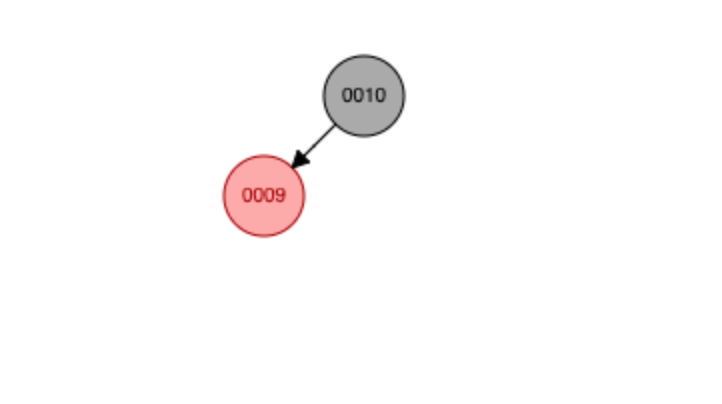
\includegraphics[width=0.5\textwidth]{Figures/q5_1.png}
  \caption{Before Insertion}
\end{figure}



After the insertion, the RBT is as below.
 \begin{figure}[hbt!]
  \centering
    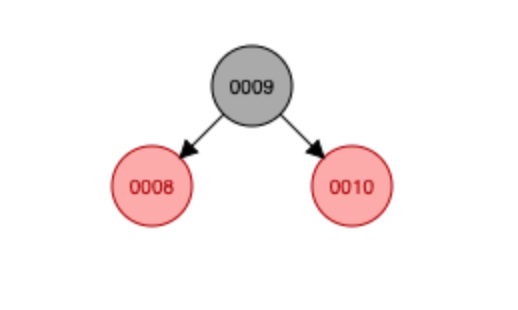
\includegraphics[width=0.5\textwidth]{Figures/q5_2.png}
  \caption{Before Insertion}
\end{figure}

After deletion, the RBT is as below.
 \begin{figure}[hbt!]
  \centering
    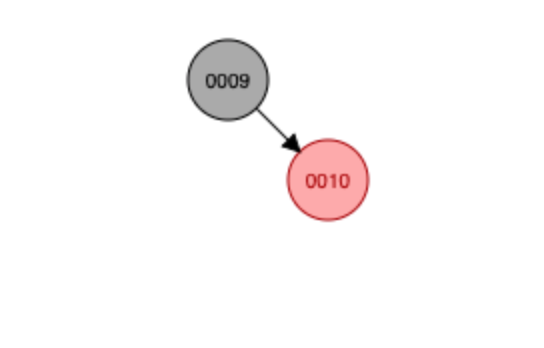
\includegraphics[width=0.5\textwidth]{Figures/q5_3.png}
  \caption{Before Insertion}
\end{figure}


For normal red-black tree, we can see that it's memoryless.

However, for left-leaning red-black tree, it keeps the memory as tested at \url{https://codetube.vn/visual/redblacktree/}. It might be attributed to the left-leaning constraint.




\section{Question 6}
\subsection{Question 6 (a)}
\lstset{
tabsize = 4, %% set tab space width
showstringspaces = false, %% prevent space marking in strings, string is defined as the text that is generally printed directly to the console
numbers = left, %% display line numbers on the left
commentstyle = \color{green}, %% set comment color
keywordstyle = \color{blue}, %% set keyword color
stringstyle = \color{red}, %% set string color
rulecolor = \color{black}, %% set frame color to avoid being affected by text color
basicstyle = \small \ttfamily , %% set listing font and size
breaklines = true, %% enable line breaking
numberstyle = \tiny,
}
\begin{lstlisting}[language = Java , frame = trBL , firstnumber = last , escapeinside={(*@}{@*)}]

public class LinearProbingHashST<Key, Value> 
{
    private int N;           // number of key-value pairs in the symbol table
    private int M = 11;      // size of linear probing table
    private Key[] keys;      // the keys
    private Value[] vals;    // the values

    public LinearProbingHashST() 
    {
        keys = (Key[])   new Object[M];
        vals = (Value[]) new Object[M];
    }

    private int mapAlphabet(String letter) 
    {
        return (letter.charAt(0) - 'A' + 1);
    }

    private int hash1(Key key) 
    {
        return mapAlphabet((String) key) % M;
    }

    private int hash2(Key key) 
    {
        double A = 0.6180339887;
        return (int) Math.floor(M * ((mapAlphabet((String) key) * A) % 1));
    }

    private int hash(Key key, int i) 
    {
        return (hash1(key) + i * hash2(key)) % m;
    }

    public void put(Key key, Value val) 
    {
        int i;
        for (i = 0; keys[hash(key, i)] != null; i++) {
            if (keys[hash(key, i)].equals(key)) {
                vals[hash(key, i)] = val;
                return;
            }
        }
        keys[hash(key, i)] = key;
        vals[hash(key, i)] = val;
        N++;
    }

    public Value get(Key key) 
    {
        for (int i = 0; keys[hash(key, i)] != null; i++) {
            if (keys[hash(key, i)].equals(key))
                return vals[hash(key, i)];
        }
        return null;
    }
}

\end{lstlisting}

\subsection{Question 6 (b)}
Note: below, $hash(k, i) =  (hash1(k) + i * hash2(k)) \mod 11$.
\begin{itemize}
\item insert E\\
hash("E", 0) = 5. That index is empty, therefore insert.\\
\item insert A\\
hash("A", 0) = 1. That index is empty, therefore insert.\\
\item insert S\\
hash("S", 0) = 8. That index is empty, therefore insert.\\
\item insert Y\\
hash("Y", 0) = 3. That index is empty, therefore insert.\\
\item insert Q\\
hash("Q", 0) = 6. That index is empty, therefore insert.\\
\item insert U\\
hash("U", 0) = 10. That index is empty, therefore insert.\\
\item insert T\\
hash("T", 0) = 9. That index is empty, therefore insert.\\
\item insert I\\
hash("I", 0) = 9. That index is full, therefore next probing.\\
hash("I", 0) = 4. That index is empty, therefore insert.\\
\item insert O\\
hash("O", 0) = 4. That index is full, therefore next probing.\\
hash("O", 1) = 6. That index is full, therefore next probing.\\
hash("O", 2) = 8. That index is full, therefore next probing.\\
hash("O", 3) = 10. That index is full, therefore next probing.\\
hash("O", 4) = 1. That index is full, therefore next probing.\\
hash("O", 5) = 3. That index is full, therefore next probing.\\
hash("O", 6) = 5. That index is full, therefore next probing.\\
hash("O", 7) = 7. That index is empty, therefore insert.\\
\item insert N\\
hash("N", 0) = 3. That index is full, therefore next probing.\\
hash("N", 1) = 10. That index is full, therefore next probing.\\
hash("N", 2) = 6. That index is full, therefore next probing.\\
hash("N", 3) = 2. That index is empty, therefore insert.\\
\end{itemize}

Trace for each insertion is showed below: 
\begin{lstlisting}
null,null,null,null,null,E,null,null,null,null,null,
null,A,null,null,null,E,null,null,null,null,null,
null,A,null,null,null,E,null,null,S,null,null,
null,A,null,Y,null,E,null,null,S,null,null,
null,A,null,Y,null,E,Q,null,S,null,null,
null,A,null,Y,null,E,Q,null,S,null,U,
null,A,null,Y,null,E,Q,null,S,T,U,
null,A,null,Y,I,E,Q,null,S,T,U,
null,A,null,Y,I,E,Q,O,S,T,U,
null,A,N,Y,I,E,Q,O,S,T,U,
\end{lstlisting}

\section{Question 7}
\begin{proof}
Let P(n) be the statement that every connected graph with n vertices has a vertex whose removal will not disconnect the graph, we will prove it with weak induction.
\medskip\\
\emph{Base Case:} n = 2.\\
When n = 2, removing any vertex will leave a single vertex and it's connected with itself. Therefore, P(2) holds.
\medskip\\
\emph{Induction Step:} When P(n) holds for all $n \ge 2$, we will prove P(n+1) holds.\\
For a connected graph with n + 1 vertices, we can arbitrarily pick n vertices. Since it's a connected graph, the n vertices are connected. With the induction hypothesis, in the n connected vertices, we can find a vertex whose removal will not disconnect the graph, named as $V_i$. We can also name the vertex which is not picked as $V_j$. \\
1. If $V_j$ is adjacent with another node in the n vertices other than $V_i$, then $V_i$ is the one we can remove. \\
2. If $V_j$ not adjacent with any node in the n vertices other than $V_i$, then it has to be adjacent $V_i$. Otherwise the graph with n + 1 vertices is not connected. In this situation, we can remove $V_j$ instead. Because it's only connected to $V_i$, the removal won't disconnect the rest graph with n vertices.
\\ 
Therefore, P(n) holds for $\forall n \ge 2 \in \mathbb{N}$ by weak induction.
\end{proof}


In the algorithm below, we assume that the graph has at least two vertices. Otherwise, it makes no sense to find such a vertex.

\begin{algorithm}
\caption{Find Vertex vis DFS}
\begin{algorithmic}[1]
\Procedure{$Get\_Vertex$}{V}
\State Initiate an empty stack S
\State Push V
\While{S is not empty}
\State current\_v $\gets$ S.top()
\State Mark current\_v as visited
\If{all vertices adjacent to current\_v are visited}
	\State \Return current\_v
\Else
	\State Push one of the unvisited vertices into stack
\EndIf
\EndWhile
\EndProcedure
\end{algorithmic}
\end{algorithm}

\section{Question 8}
To produce a topological order, we need to put all start nodes (with indegree 0) into the queue first. After that, if we used only the given algorithm, we could have generated wrong topological order for some graph as shown below.

 \begin{figure}[hbt!]
  \centering
    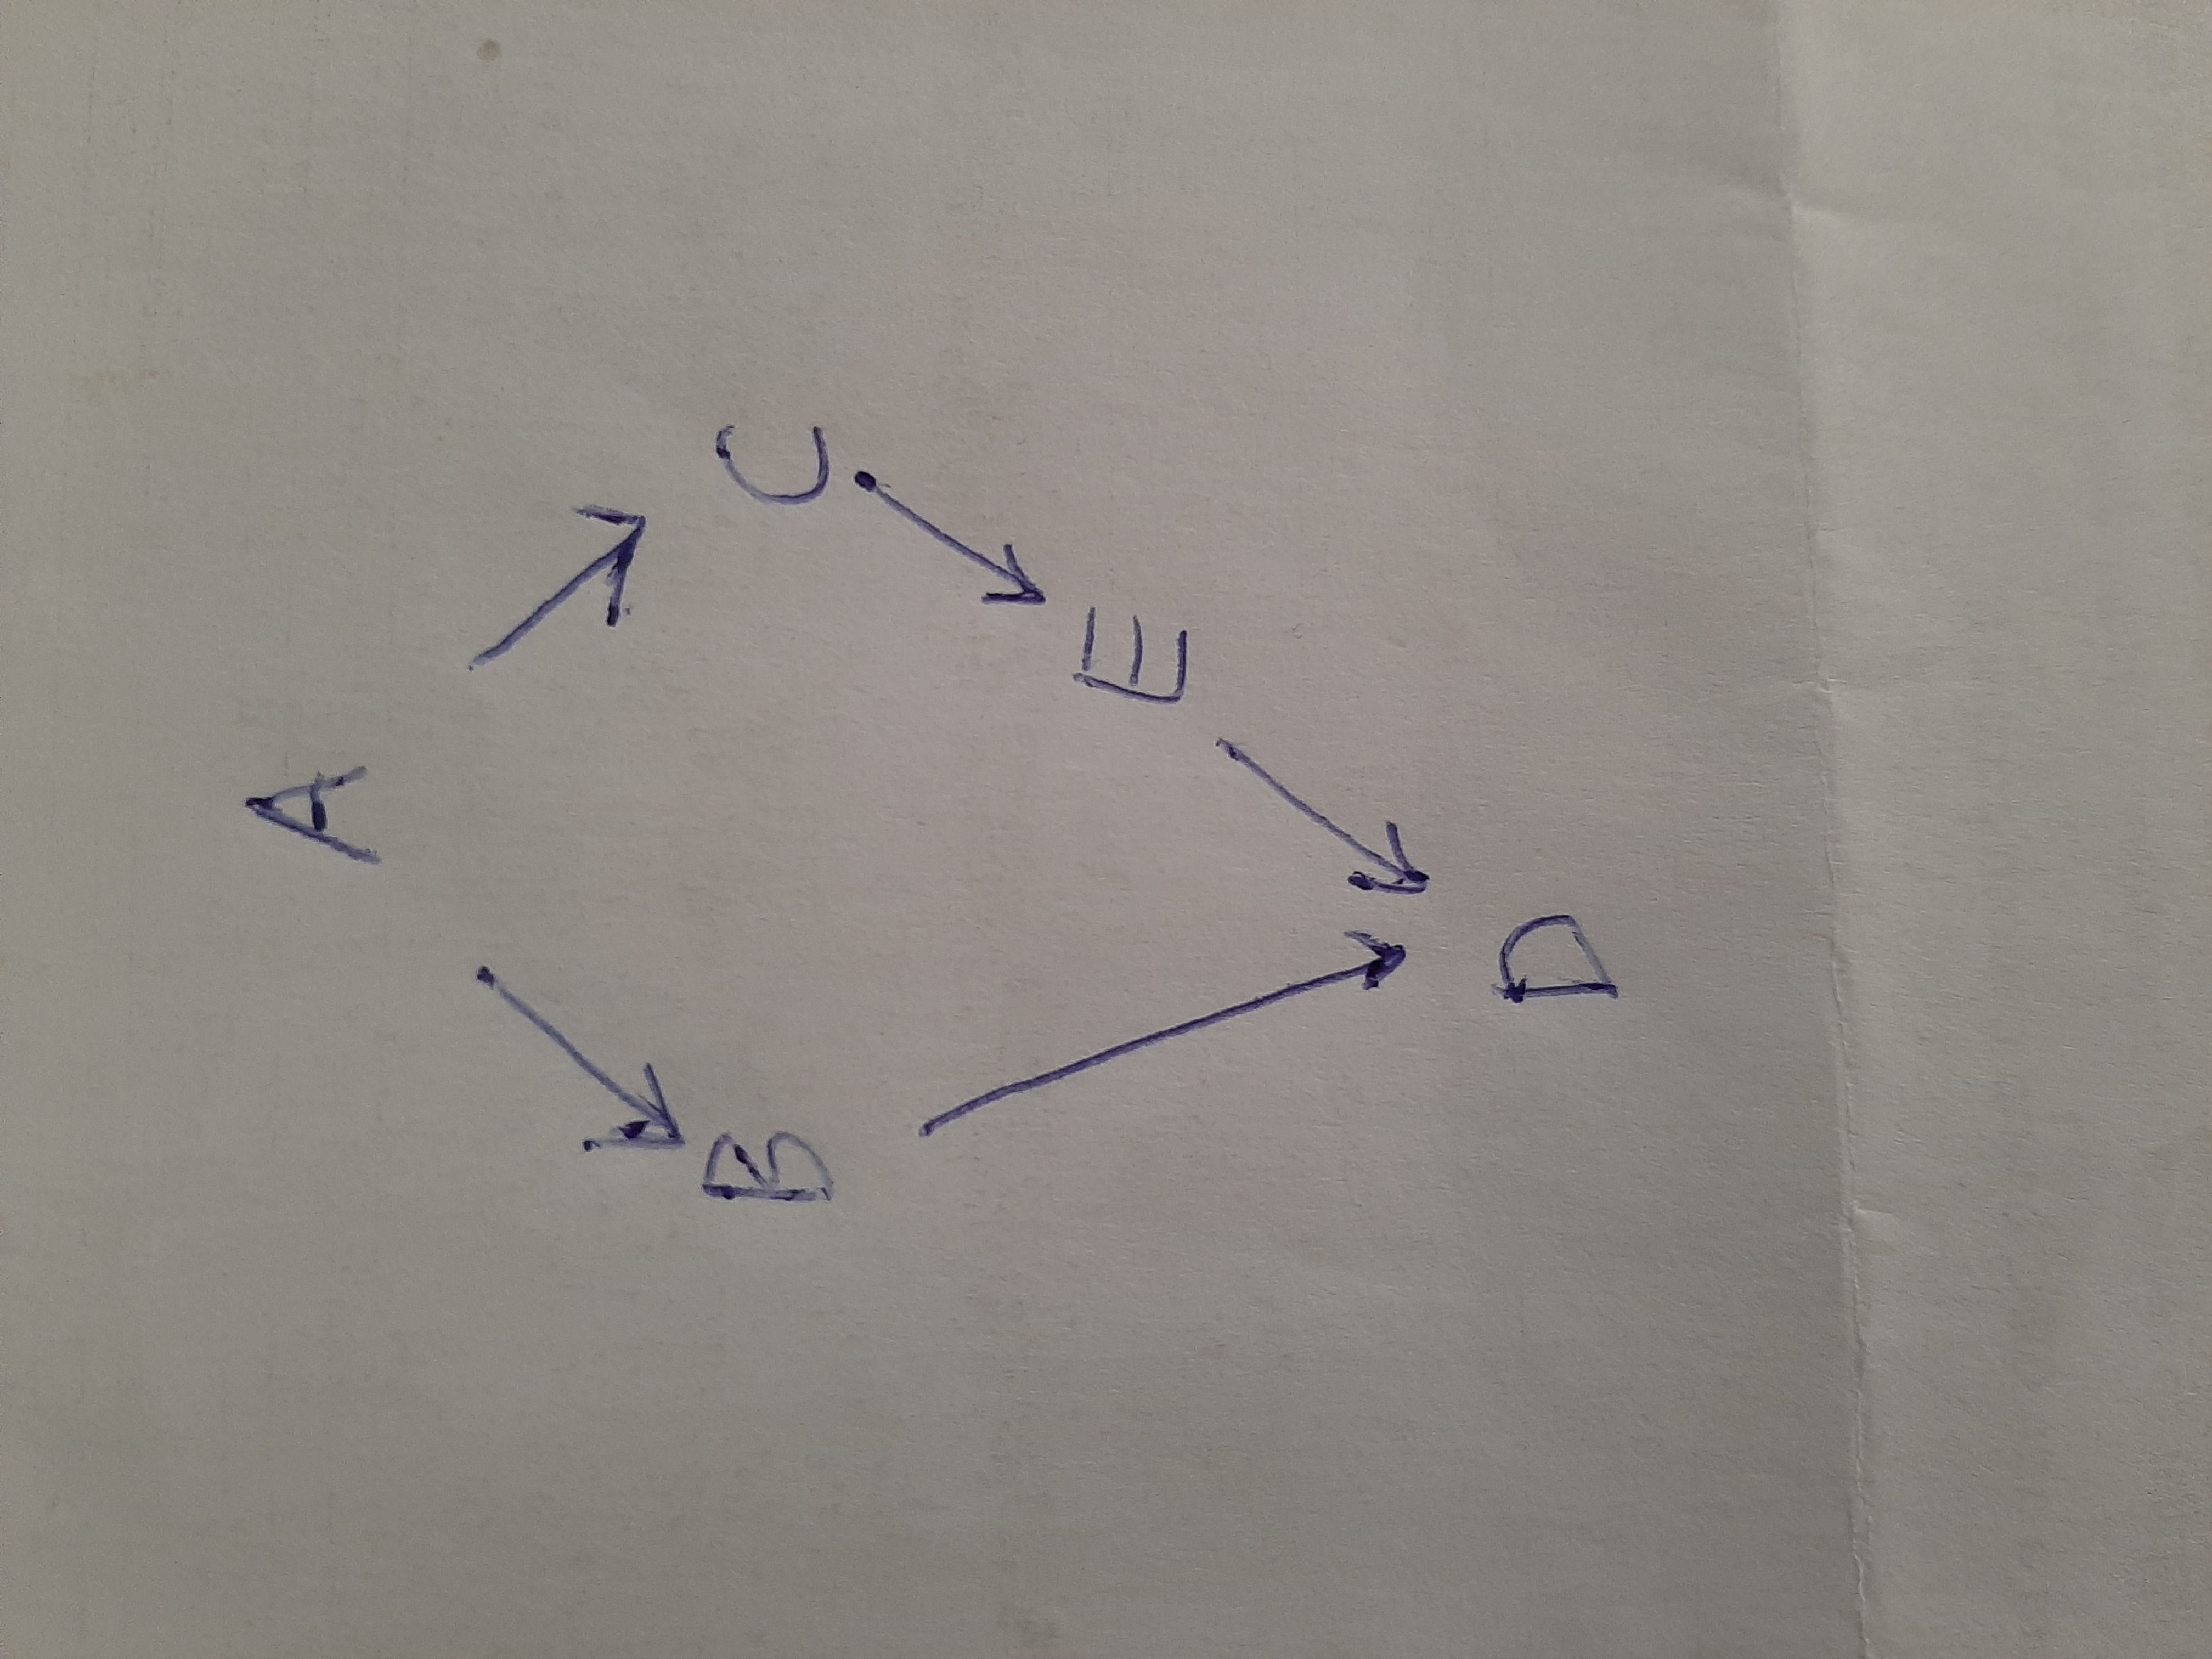
\includegraphics[width=0.5\textwidth, angle =-90]{Figures/q8.jpg}
  \caption{Directed Acyclic Graph}
\end{figure}

\newpage
With BFS, we'll enqueue A  and mark its distance as 0. Then we'll dequeue A and enqueue B and C and mark the distance of B and C as 1. After that, we'll dequeue B and enqueue D into the queue. However, D should be behind E in topological order.
This situation happens because in the algorithm we don't check the in-degree of each node, which is the fault of the given algorithm based on BFS. With BFS, If a node's in-degree is greater than 1, it should not be inserted. Instead, its in-degree should be reduced by 1 for each predecessor. We should only enqueue a node when its in-degree drops to 1, which means all of its predecessors are visited.  


\end{document}




